\documentclass{article}
\usepackage[utf8]{inputenc}
\usepackage{graphicx}

\usepackage[ruled, lined, linesnumbered, commentsnumbered, longend]{algorithm2e}
\usepackage{xcolor}
\usepackage{mathtools}
\usepackage[]{algorithm2e}
\usepackage[a4paper, total={170mm,257mm},left=25mm,right=25mm, top=20mm,]{geometry}
\title{Report for Sokoban game solution with Path-finding Algorithms}
\author{\textbf{Tan Pham Ngoc}\\
Faculty of Computer Science, University of Information Technology\\
\small ngctnnnn@gmail.com}
\date{March 2021}

\begin{document}

\maketitle

\section{How is Sokoban game modelized ?} 

\textit{Sokoban game} is constructed as one agent, which is Sokoban, in her mission pushing all the boxes into the goals. The game is initialized as many given maps or "levels", in which \textbf{"$\#$"} as the \textit{walls}, \textbf{"B"} as the \textit{boxes}, \textbf{"."} as the \textit{goals}, " " as the \textit{free space} and \textbf{"$\&$"} as the \textit{initialized position} for Sokoban in the game.\\

The game shall meet its end once all the boxes are put into their correct places (\textit{the goals}, in others way).\\

The \textit{state space} of the game is the position of the Sokoban itself and the position of the boxes.\\

There are four \textit{legal actions} in the game of Sokoban, which are go up, go down, go left and go right. However, for a more details saying, let us consider the game has totally 8 legal actions, which are \textit{go left}, \textit{go right}, \textit{go up}, \textit{go down} and \textit{interact with the boxes} \\

The successor function of this game is defined as the location of Sokoban after taking one legal actions from the action space, or the position of both Sokoban and the box in the event of Sokoban's choice to push the boxes.

\section{A brief comparison between 3 others path finding algorithms}
\subsection{Depth first search}
\textit{Depth first search} (DFS) is the only algorithm set up in the auto mode. For a closer look at the difference between path finding algorithms, let us take a look at the DFS algorithm.\\

DFS algorithm takes the idea of backtracking, it involves exhaustive searches of all the node by moving forward, else by backtracking. The advantage of using DFS in this modelized game is that the answer might be found quickly, it does not guarantee the quality, despite. And a foreseen consequence for using this algorithm as the solution is that the answer is unnecessary long, even if for just a simple test. And I shall clarify this comment in the sections below.

\subsection{Breadth first search}
\textit{Breadth first search} (BFS) is a traversed algorithm where you start traversing from a selected node and traverse the graph layer-wise thus exploring the neighbour nodes (nodes which are directly connected to source node). You must then move towards the next-level neighbour nodes.\\

When constructing the algorithm, I utilize the code of DFS given previously with a micro change, in which I change the deque from pop (here its mean pop the rightmost element) into pop the leftmost element in the deque. This is due to the basic difference between two different concepts of DFS and BFS.\\

The answer given by BFS algorithm is by far better than DFS significantly, where it fixes the drawbacks of the DFS algorithm - unnecessarily long answers for a simple state.\\

In details, we might pick a certain map in the game and let us take a closer look for a detailed efficiency between DFS and BFS - map 3.
The map is described as below:
\begin{figure}[h!]
  \centering
  \begin{minipage}[b]{0.4\textwidth}
    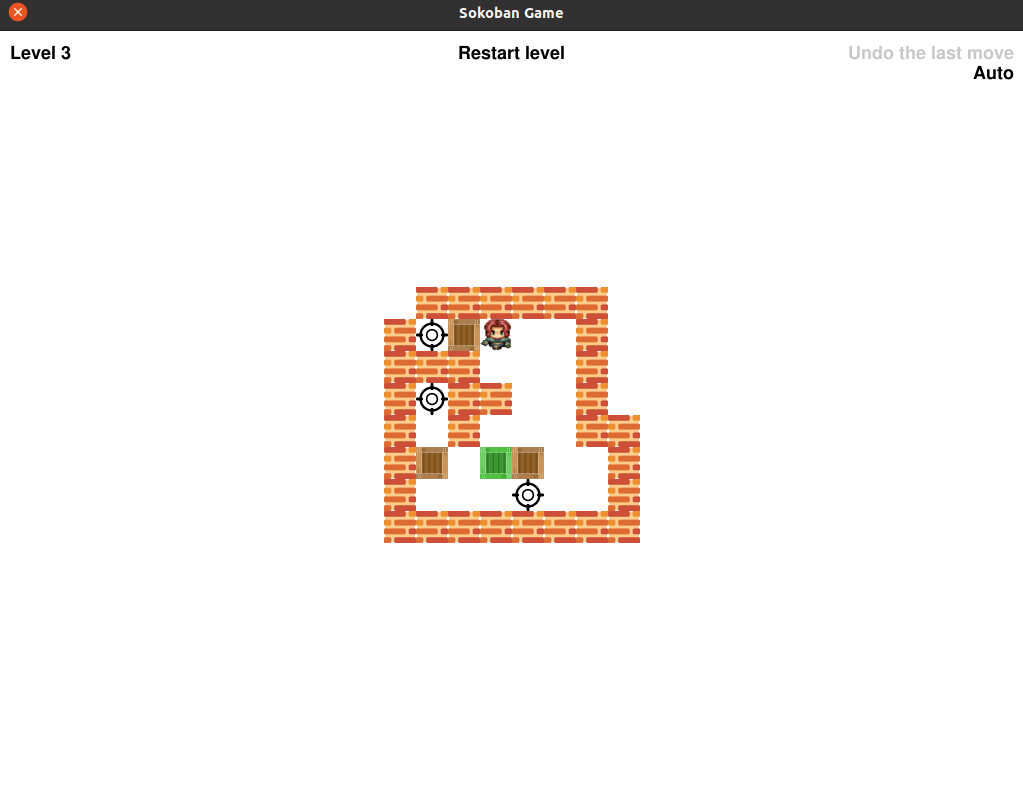
\includegraphics[width=\textwidth]{Level 3.png}
    \caption{Level 3 description}
  \end{minipage}
  \hfill
\end{figure}\\

The answer of DFS is:
    [r, r, d, l, d, r, d, l, l, D, R, l, l, d, l, U, r, r, r, d, r, r, u, L, r, d, l, l, L, r, r, r, u, l, u, l, l, d, R, l, l, l, d, R, l, u, r, r, r, d, r, r, u, L, r, d, l, l, U, r, r, d, l, l, L, r, r, r, u, l, l, l, l, l, d, R, R, R, l, l, l, u, r, r, r, r, r, d, L, r, u, l, l, l, l, l, U, d, r, r, r, r, r, d, l, L, r, r, u, l, l, l, l, l, d, r, R, R, l, l, l, u, r, r, r, r, r, d, L, r, u, l, l, l, u, R, l, d, r, r, r, d, l, L, r, r, u, l, l, l, l, l, d, r, R, R, l, l, l, u, r, r, r, r, r, d, L, r, u, l, l, l, u, r, u, r, u, l, l, u, L, r, r, r, d, l, d, d, l, d, r, r, r, d, l, L, r, r, u, l, l, l, l, l, d, r, R, R, l, l, l, u, r, r, r, r, r, d, L, r, u, l, U, l, l, d, r, r, r, d, l, L, r, r, u, l, l, l, l, l, d, r, R, R, l, l, l, u, r, r, r, r, r, d, L, r, u, l, l, l, u, r, r, U, l, d, r, d, r, d, l, L, r, r, u, l, l, l, l, l, d, r, R, R, l, l, l, u, r, r, r, r, r, d, L, r, u, l, l, l, u, r, r, u, l, u, l, u, r, r, D, D, l, d, l, d, r, r, r, d, l, L, r, r, u, l, l, l, u, r, u, r, D, l, l, d, r, d, r, r, u, L, r, d, l, l, L, r, r, r, u, l, u, l, l, d, R, l, l, l, d, R, l, u, r, r, r, d, L, r, r, r, u, L, r, d, l, l, l, u, l, l, d, R, R, R, l, l, l, u, r, r, u, r, r, d, r, d, L, r, u, l, L]\\
    
Meanwhile, the answer of BFS is: $\left[\text{L, r, d, r, d, d, D, L, d, l, l, U, U, d, R}\right]$\\

On the contrary, despite the major efficiency in the algorithm of breadth first search algorithm, it is still not able to solve map 5, which might be the most difficult map in the game. That is, thus, the reason for why we have the third path finding algorithm.
\subsection{Uniform cost search}
As mentioned before, despite the powerful and major advances in breadth first search, the algorithm itself can not solve the problem itself (or perhaps it could, with a huge amount of time or an enormous processor. This can be dissolved successfully, fortunately, through the use of a more advanced algorithm - \textit{Uniform cost search}.\\

The main idea behind the concept of Uniform cost search (UCS) algorithm is to compute the past costs in order of increasing past cost. To make this efficient, we need to make an important assumption that all action costs are non-negative. UCS and Dijikstra's algorithm has many similarities, however, UCS algorithm takes input as a search problem, which implicitly defines a large and even infinite graph, whereas Dijkstra’s algorithm (in the typical exposition) takes as input a fully concrete graph.\\ 

The clearest evidence for the surpassing power of this algorithm is to give it through one hard problem, which can not be solved easily by 2 others algorithms: BFS and DFS.\\

Surprisingly, uniform cost search solves it without a doubt, within just a little time to take: 63 seconds in details in Intel@Corei5 processor. What is more, the solution given by UCS share the similarities with the BFS, but with a faster time to take.\\

Hence, it is clear to tell that Uniform cost search is by far the best path-finding algorithm among the others, which are depth-first search and breadth-first search.
\end{document}
